\section{Grim Reaper Class Weapons}

\subsubsection{Scythe of the Unmaker}

The Scythe of the Unmaker is an ancient Scythe of legend. It is said that this weapon was wielded by the first Grim Reaper to exist. It is claimed that this Reaper stole the scythe from a god, Argus the Unmaker. The scythe is said to contain all of the souls of those slain by it. This is  where the power of the scythe is from. The wielder of the scythe is said to forever be cursed with the burdens of the souls it contains and will slowly be corrupted by its power.

\begin{center}
	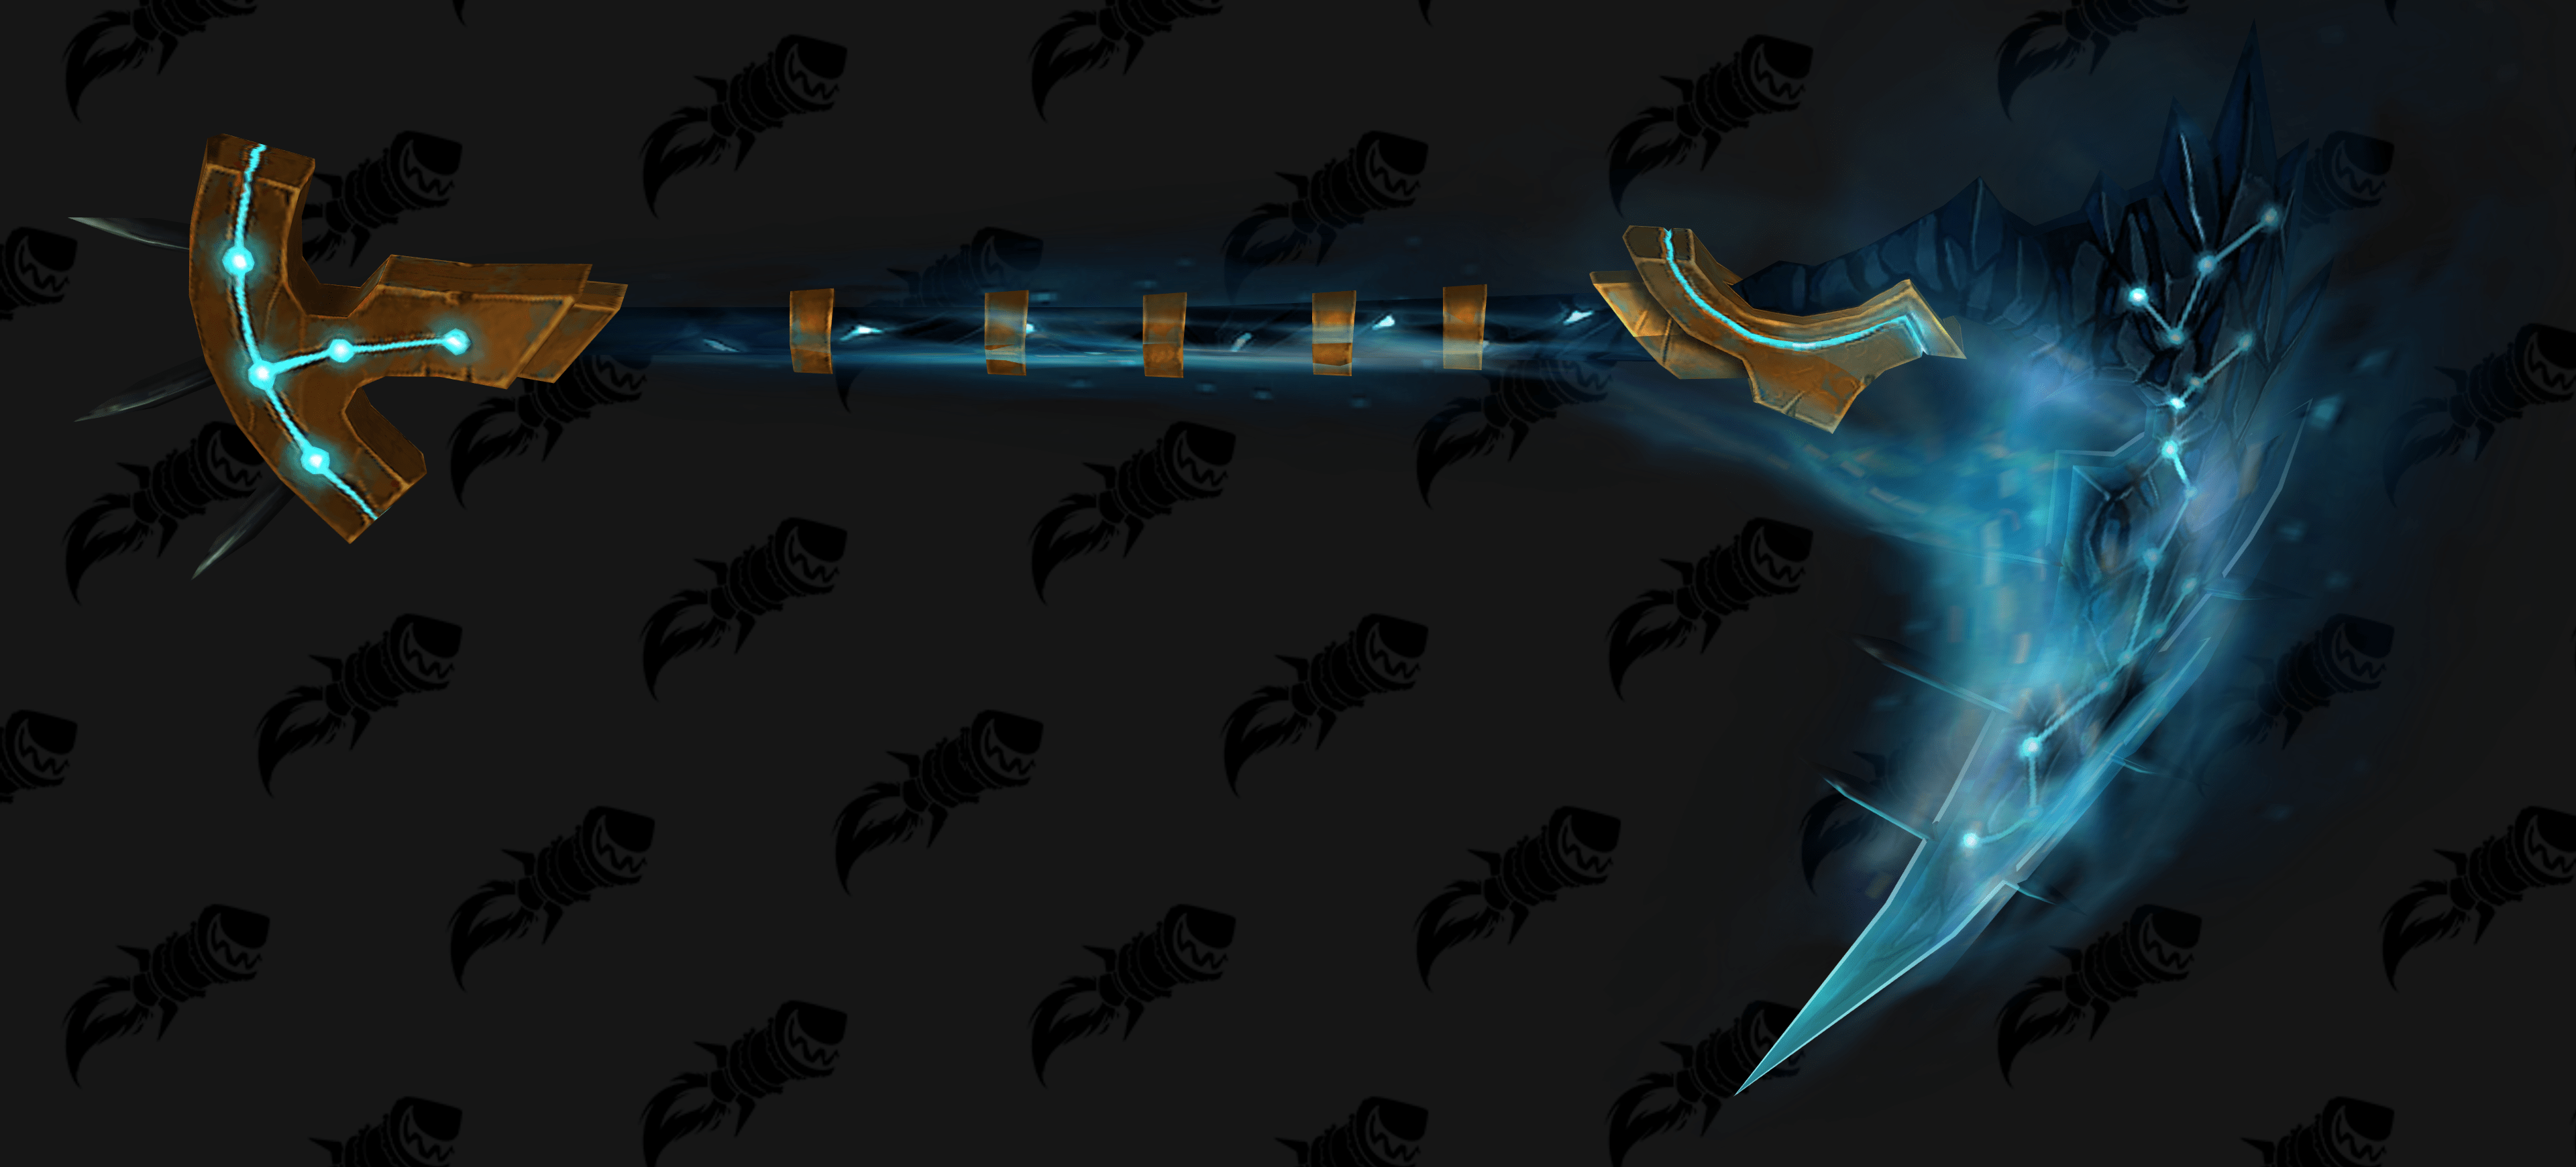
\includegraphics[width=\linewidth]{img/weapons/1213012.png}
\end{center}

\subsubsection{Potential}

The Scythe of the Unmaker seeks the souls of victims. It can try to influence the wielder to want to attack a target if it so desires the soul of them.

\begin{commentbox}{Scythe of the Unmaker\footnote{Weapon (scythe), artifact (requires attunement by a Grim Reaper)}}
	You gain a +3 bonus to attack and damage rolls made with this magic weapon. When you hit an enemy you will deal 2d4 psychic damage and 2d4 necrotic damage. The damage will change to d8's if the target has a good alignment.
	
	The target of a melee attack of these blades must make a constitution saving throw. On a fail, they take 4d6 psychic damage. The DC for this save is the wielders level + their constitution.
	
	Any. When the wielder rolls a 20 against a character with good alignment the wielder must a d100 roll. If the roll is less than half the wielders lvl then the fiend or undead will have it's soul removed and become lifeless immediately.
	
	If a Grim Reaper of an good alignment tries to attune to The scythe they have to make a d20 roll. 
	\begin{enumerate}
		\item Chaotic good: At a 12 or below The scythe will reject you and deal 3d10 necrotic damage and 2d10 psychic damage. At a 12 or above you over power the will of the weapon and make it yours.
		\item Neutral good: At a 16 or below The scythe will reject you and deal 3d10 necrotic damage and 2d10 psychic damage. At a 16 or above you over power the will of the weapon and make it yours.
		\item Lawful good: At a 18 or below The scythe will reject you and deal 3d10 necrotic damage and 2d10 psychic damage. At a 19 or 20 you over power the will of the weapon and make it yours.
	\end{enumerate}
	
	Proficiency with a scythe allows you to add your proficiency bonus to the attack roll for any attack you make with it.
\end{commentbox}

\subsubsection{Finding the Scythe of the Unmaker}

The Scythe of the Unmaker is located in an ancient and haunted graveyard deep in the Pluvian Forest. The graveyard is centuries old and buried within an underground bog in the caverns of a large mountain. The scythe is help in the grave with an undead warlock necromancer. This necromancer found the scythe and tried to harness its power but utterly failed. After studying the scythe the necromancer tried to tap into its potential to resurrect fallen spirits from this graveyard, but instead was consumed in the process. In his death, the necromancer became entrapped by the power of the scythe becoming eternally dammed to be a keeper of the graveyard and protector of the scythe. When entering the graveyard, a horde of undead will awaken and attack anyone who dares intrude on the graves. The fallen necromancer will command them in protecting the scythe. If the necromancer is killed, the undead he commands will also fall.

\begin{monsterbox}{Necromancer}
	\begin{hangingpar}
		\textit{Medium Undead, lawful evil}
	\end{hangingpar}
	\dndline%
	\basics[%
	armorclass = 16,
	hitpoints  = 82,
	speed      = 30 ft
	]
	\dndline%
	\stats[
	STR = \stat{9}, % This stat command will autocomplete the modifier for you
	DEX = \stat{12},
	CON = \stat{14},
	INT = \stat{16},
	WIS = \stat{22},
	CHA = \stat{10}
	]
	\dndline%
	\details[%
	% If you want to use commas in these sections, enclose the
	% description in braces.
	% I'm so sorry.
	languages = {Common, undead},
	challenge = 6
	]
	\dndline%
	damage resistance = Necrotic, Poison
	
	condition immunities = Exhaustion, Petrified, Poisoned, Paralyzed, Feared	
	
	Senses = Passive Perception 20
	
	\dndline%
	\begin{monsteraction}[Horrify]
		All creatures within 60 ft. of you must make a DC18 constitution save. On a fail, they become frightened. On a success nothing happens and they become immune to your frightening glare for 24 hours.
	\end{monsteraction}	
	\begin{monsteraction}[Multiattack]
		You can take two attack actions per turn.
	\end{monsteraction}
	\monstersection{Actions}
	\begin{monsteraction}[Life Tap]
		As an action, you can make a melee spell attack against a living creature, dealing necrotic damage equal to 2d8 + your Charisma modifier on a hit. You gain temporary hit points equal to the amount of necrotic damage dealt. If this feature kills the creature, you gain twice as many temporary hit points from using this feature.
	\end{monsteraction}	
	\begin{monsteraction}[Melee Attack]
		Melee scythe attack. +5 to hit.
	\end{monsteraction}	
	\begin{monsteraction}[Confuse Soul]
		You blacken the mind of a living target. The target must make a DC16 wisdom save or lose a turn as their soul is struggling to stay connected to their physical bodies.
	\end{monsteraction}		
\end{monsterbox}


\begin{monsterbox}{Soulless Zombie}
	This character design is adapted from https://roll20.net/compendium/dnd5e/Zombie\#content
	\begin{hangingpar}
		\textit{medium undead, neutral evil}
	\end{hangingpar}
	\dndline%
	\basics[%
	armorclass = 8,
	hitpoints  = 22,
	speed      = 20 ft
	]
	\dndline%
	\stats[
	STR = \stat{13}, % This stat command will autocomplete the modifier for you
	DEX = \stat{6},
	CON = \stat{16},
	INT = \stat{3},
	WIS = \stat{6},
	CHA = \stat{5}
	]
	\dndline%
	\details[%
	% If you want to use commas in these sections, enclose the
	% description in braces.
	% I'm so sorry.
	languages = {All, cannot speak},
	challenge = 1/4
	]
	\dndline%
	saving throws = Wisdom +0
	
	damage immunities = Poison
	
	condition immunities = Poisoned	
	
	Senses = Darkvision 60 ft., passive Perception 8
	\dndline%
	\begin{monsteraction}[Undead Fortitude]
		If damage reduces the zombie to 0 hit points, it must make a Constitution saving throw with a DC of 5+the damage taken, unless the damage is radiant or from a critical hit. On a success, the zombie drops to 1 hit point instead.
	\end{monsteraction}	
	\monstersection{Actions}
	\begin{monsteraction}[Slam]
		Melee Weapon Attack: +3 to hit, reach 5 ft., one target. Hit: (1d4 + 1) bludgeoning damage. 
	\end{monsteraction}		
\end{monsterbox}